\documentclass[11pt,a4paper]{article}
\usepackage{amsmath,amsthm,amsfonts,amssymb,amscd}
\usepackage{enumerate} 
\usepackage{physics}
\usepackage{enumerate}
\usepackage{fancyhdr}
\usepackage{hyperref}
\usepackage{graphicx}
\usepackage{xurl}
\hypersetup{colorlinks,
    linkcolor=blue,
    citecolor=blue,      
    urlcolor=blue,
}

\oddsidemargin0.1cm 
\evensidemargin0.8cm
\textheight22.7cm 
\textwidth15cm \topmargin-0.5cm

\newtheorem{theorem}{Theorem}
\newtheorem{corollary}{Corollary}
\newtheorem{lemma}{Lemma}
\newtheorem{proposition}{Proposition}

\theoremstyle{definition}
\newtheorem{remark}{Remark}
\newtheorem{definition}{Definition}
\newtheorem{observation}{Observation}
\newtheorem{note}{Note}
\newtheorem{hope}{Hope}
\newtheorem{warning}{Warning}
\newtheorem{problem}{Problem}
\newtheorem{fear}{Fear}
\newtheorem{question}{Question}

\newcommand{\Z}{\mathbb{Z}}
\newcommand{\R}{\mathbb{R}}
\newcommand{\C}{\mathbb{C}}
\newcommand{\Q}{\mathbb{Q}}
\newcommand{\A}{\mathbb{A}}

\usepackage{listings}
\usepackage{xcolor}

\definecolor{codegreen}{rgb}{0,0.6,0}
\definecolor{codegray}{rgb}{0.5,0.5,0.5}
\definecolor{codepurple}{rgb}{0.58,0,0.82}
\definecolor{backcolour}{rgb}{0.95,0.95,0.92}

\lstdefinestyle{mystyle}{
    backgroundcolor=\color{backcolour},   
    commentstyle=\color{codegreen},
    keywordstyle=\color{magenta},
    numberstyle=\tiny\color{codegray},
    stringstyle=\color{codepurple},
    basicstyle=\ttfamily\footnotesize,
    breakatwhitespace=false,         
    breaklines=true,                 
    captionpos=b,                    
    keepspaces=true,                 
    numbers=left,                    
    numbersep=5pt,                  
    showspaces=false,                
    showstringspaces=false,
    showtabs=false,                  
    tabsize=2
}

\lstset{style=mystyle}

\newcommand{\MultiSet}{\mathrm{MultiSet}}
\newcommand{\len}{\mathrm{len}}
\newcommand{\din}{\texttt{d\_in}}
\newcommand{\dout}{\texttt{d\_out}}
\newcommand{\Relation}{\texttt{relation}}
\newcommand{\X}{\mathcal{X}}
\newcommand{\Y}{\mathcal{Y}}
\newcommand{\U}{\texttt{U}}
\newcommand{\True}{\texttt{True}}
\newcommand{\False}{\texttt{False}}
\newcommand{\clamp}{\texttt{clamp}}
\newcommand{\function}{\texttt{function}}
\newcommand{\float}{\texttt{float }}
\newcommand{\questionc}[1]{\textcolor{red}{\textbf{Question:} #1}}

\newcommand{\silvia}[1]{{ {\color{blue}{(silvia)~#1}}}}
\newcommand{\grace}[1]{{ {\color{purple}{(grace)~#1}}}}
\newcommand{\connor}[1]{{ {\color{teal}{(connor)~#1}}}}

\newcommand{\todo}{{\textcolor{red}{TODO }}}


\title{Privacy Proofs for OpenDP: Mean}
\author{S\'ilvia Casacuberta}
\date{Summer 2021}

\begin{document}

\maketitle

\tableofcontents

\section{Algorithm Implementation}
\subsection{Code in Rust}
The current OpenDP library contains the transformation \texttt{make\_bounded\_mean} implementing bounded sum with known $n$. This is defined in lines 11-33 of the file \texttt{mean.rs} in the Git repository\footnote{As of July 27, 2021.} (\url{https://github.com/opendp/opendp/blob/main/rust/opendp/src/trans/mean.rs#L11-L33}).

\begin{figure}[ht]
    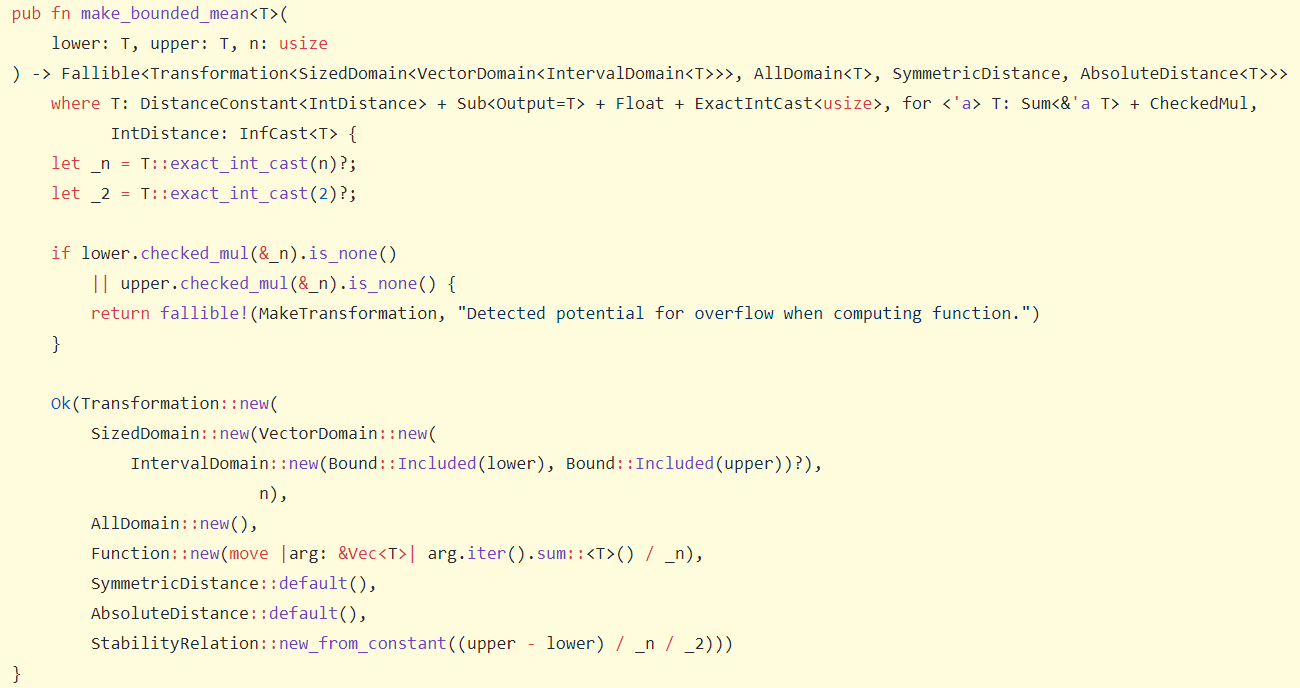
\includegraphics[width=15cm]{mean_rust.png}
    \centering
    \label{fig:code}
\end{figure}

% what do to with n? Take it as input to T(x)?
% Is it correct to say x_i? I mean the i-th element in the multiset

\subsection{Pseudocode in Python}
We present a simplified Python-like pseudocode of the Rust implementation below. The necessary definitions for the pseudocode can be found at \href{https://www.overleaf.com/project/60d215bf90b337ac02200a99}{``List of definitions used in the pseudocode"}.

\subsubsection*{Preconditions}
To ensure the correctness of the output, we require the following preconditions:

\begin{itemize}
    \item \textbf{User-specified types:}
    \begin{itemize}
        \item Variable \texttt{n} must be of type \texttt{usize}.
        \item Type \texttt{T} must have traits \texttt{DistanceConstant(IntDistance)}, \texttt{TotalOrd},\footnote{For now, the OpenDP library only implements \texttt{PartialOrd}, but \texttt{TotalOrd} will soon be implemented. Then, \texttt{TotalOrd} will be redundant, since the trait \texttt{TotalOrd} is part of the trait \texttt{DistanceConstant}.} \texttt{Sub(Output=T)}, \texttt{ExactIntCast(usize)}, \texttt{CheckedMul}, \texttt{Sum(Output=T)}, and \texttt{Float}. 
        \item \texttt{InfCast(T)}. \questionc{Same comment as in \texttt{make\_count} and \texttt{MakeBoundedSumN} -- this is not needed for the proof.}
    \end{itemize}
\end{itemize}

\subsubsection*{Postconditions}
\begin{itemize}
    \item Either a valid \texttt{Transformation} is returned or an error is returned.
\end{itemize}

\begin{lstlisting}[language=Python, escapechar=|]
def MakeBoundedMean(L: T, U: T, n: usize):
    input_domain = SizedDomain(VectorDomain(IntervalDomain(L, U)))
    output_domain = AllDomain(T)
    input_metric = SymmetricDistance()
    output_metric = AbsoluteDistance(T)
    
    n_ = exact_int_cast(n, T)
    
    if checked_mul(L, n_).is_none or checked_mul(U, n_).is_none: 
        raise Exception('Potential overflow') |\label{line:max}|
    
    def relation(d_in: u32, d_out: T) -> bool: |\label{line:rel}|
        return d_out >= inf_cast(d_in, T)*(U-L) / n_ / exact_int_cast(2, T)
    
    def function(data: Vec[T]) -> T: |\label{line:fn}|
        return (data.iter().sum()) / n_ |\label{line:sum}|
    
    return Transformation(input_domain, output_domain, function, input_metric, output_metric, stability_relation = relation)
\end{lstlisting}

\section{Proof}
\subsection{Symmetric Distance}
\begin{theorem}
    For every setting of the input parameters \texttt{(L, U, n)} to \texttt{MakeBoundedMean}, the transformation returned by \texttt{MakeBoundedMean} has the following properties:
    \begin{enumerate}
        \item \textup{(Appropriate output domain).} For every element $v$ in \texttt{input\_domain}, $\function(v)$ is in \texttt{output\_domain}. % Prof. Vadhan said on 29/6 to leave it as this for now, but maybe in the future we add to the theorem statement what exactly the input domain and output domain are (although of course we already say this in the proof)
        \item \textup{(Domain-metric compatibility).} The domain \texttt{input\_domain} matches one of the possible domains listed in the definition of \texttt{input\_metric}, and likewise \texttt{output\_domain} matches one of the possible domains listed in the definition of \texttt{output\_metric}.
        
        \item \textup{(Stability guarantee).} For every pair of elements $v, w$ in \texttt{input\_domain} and for every pair $(\din, \dout)$, where $\din$ is of the associated type for \texttt{input\_metric} and $\dout$ is the associated type for \texttt{output\_metric}, if $v,w$ are $\din$-close under \texttt{input\_metric} and $\Relation(\din, \dout) = \True$, then $\function(v)$, \texttt{function}$(v)$ are $\dout$-close under \texttt{output\_metric}.
    \end{enumerate}
\end{theorem}

\begin{proof}
    \textbf{(Appropriate output domain).} In the case of \texttt{MakeBoundedMean}, this corresponds to showing that for every vector $v$ in \texttt{SizedDomain(VectorDomain(IntervalDomain (L, U)), n)}, where \texttt{L} and \texttt{U} have type \texttt{T}, then \texttt{function}$(v)$ belongs to \texttt{AllDomain(T)}. 
    The output correctness follows from the type signature of \texttt{function} as defined in line \ref{line:fn} and from the overflow check done through the \texttt{checked\_mul} function in line \ref{line:max}. The latter ensures that \texttt{function(v)} is contained within the interval \texttt{[get\_min\_value(T), get\_max\_value(T)]}, and hence prevents any overflow from occurring in line \ref{line:sum}. Otherwise, an exception for potential overflow will be raised, as described in line~\ref{line:max}. The former automatically enforces that \texttt{function(v)} has type \texttt{T}. Since the Rust code successfully compiles, by the type signature the appropriate output domain property must hold. Otherwise, the code will raise an exception for incorrect input type.
    
    \questionc{Should I say something about the \texttt{exact\_int\_cast} check?}
    
    \smallskip
    \textbf{(Domain-metric compatibility).} For \texttt{MakeBoundedMean}, this corresponds to showing that \texttt{SizedDomain(VectorDomain(IntervalDomain (L, U)), n)} is compatible with symmetric distance, and that \texttt{AllDomain(T)} is compatible with absolute distance. The latter follows directly from the list of compatible domains in the definition of absolute distance, as described in \href{https://www.overleaf.com/project/60d215bf90b337ac02200a99}{``List of definitions used in the pseudocode"}. The former follows from the compatibility of symmetric distance and \texttt{VectorDomain(D)} as stated in the definition of symmetric distance along with the fact that \texttt{SizedDomain(VectorDomain(D))} is a subdomain of \texttt{VectorDomain(D)}. By Theorem 2.1 in \href{https://www.overleaf.com/project/60d215bf90b337ac02200a99}{``List of definitions used in the pseudocode"}, this implies that \texttt{SizedDomain(VectorDomain(D))} is compatible with symmetric distance as well. 
    
    \silvia{Flag: this is an example of the subdomain issues that we have been discussing during the week of July 19. Hence this paragraph might need some phrasing updates when the compatibility pairing constructor and the subdomain trait are implemented.}
    
    \smallskip
    \textbf{(Stability guarantee).} Throughout the stability guarantee proof, we can assume that $\function(v)$ and $\function(w)$ are in the correct output domain, by the \textit{appropriate output domain property} shown above. 
    
    Since by assumption $\Relation(\din, \dout) = \True$, by the \texttt{MakeBoundedMean} stability relation (as defined in line~\ref{line:rel} in the pseudocode), we have that $\dout \geq \din \cdot (\U - \texttt{L})/2\texttt{n}$. Moreover, $v, w$ are assumed to be $\din$-close. By the definition of the symmetric difference metric, this is equivalent to stating that $d_{Sym}(v, w) = |\MultiSet(v) \Delta \MultiSet(w)| \leq \din$.

    Further, applying the histogram notation,\footnote{See \textit{A Programming Framework for OpenDP}, footnote 1 in page 3. Note that there is a bijection between multisets and histograms, which is why the proof can be carried out with either notion. For further details, please consult \url{https://www.overleaf.com/project/60d214e390b337703d200982}.}  it follows that
    \[
        d_{Sym}(v, w) = \lVert h_{v} - h_{w}\rVert_1 = \sum_z |h_v(z) - h_w(z)| \leq \din.
    \]
    We want to show that
    \[
        d_{Abs}(\function(v), \function(w)) \leq d_{Sym}(v, w) \cdot \dfrac{\texttt{U-L}}{2\texttt{n}}.
    \]
    This would imply that
    \begin{equation}\label{eq:abs1}
        d_{Abs}(\function(v), \function(w)) \leq d_{Sym}(v, w) \cdot \dfrac{\texttt{U-L}}{2\texttt{n}} \leq \din \cdot \dfrac{\texttt{U-L}}{2\texttt{n}},
    \end{equation}
    and by the stability relation this will imply that
    \begin{equation}\label{eq:abs2}
        d_{Abs}(\function(v), \function(w)) \leq \dout,
    \end{equation}
    as we want to see. 
\end{proof}

%\newpage

\subsection{First proof: using the path property (adjacent pairs approach)}

To show that $d_{Abs}(\function(v), \function(w)) \leq d_{Sym}(v, w) \cdot \frac{\texttt{U-L}}{2\texttt{n}}$, we will use the three lemmas described in the section ``The path property of symmetric distance on sized domains" from the document \href{https://www.overleaf.com/project/60d214e390b337703d200982}{``List of definitions used in the proofs"}. With these three lemmas, which are applicable to \texttt{MakeBoundedMean} because \texttt{input\_domain} is a a sized domain and \texttt{input\_metric} is symmetric distance, it suffices to show the following: For all vectors $x, y \in$ \texttt{input\_domain} such that $d_{Sym}(x, y) = 2$, it follows that 
\[
d_{Abs}(\texttt{function}(x), \texttt{function}(y)) \leq \dfrac{\texttt{U} - \texttt{L}}{\texttt{n}}.
\]
By Lemma 4.2 from \href{https://www.overleaf.com/project/60d214e390b337703d200982}{``List of definitions used in the proofs"}, we know that vectors $x, y$ only differ on one element, given that, by assumption, $d_{Sym}(x, y) = 2$. Wlog, let this different element be the $k$-th element of $x$ and $y$, where $x_k = \alpha$, $y_k = \beta$ with $\alpha \neq \beta$.\footnote{The first element of a vector is indexed by 0.} Then,
\[
    d_{Abs}(\texttt{function}(x), \texttt{function}(y)) = |\texttt{function}(x) - \texttt{function}(y)| = 
\]
\[
    = \Big|\dfrac{1}{\texttt{n}}\sum_{i=0}^{\texttt{n}-1}x_i - \dfrac{1}{\texttt{n}}\sum_{i=0}^{\texttt{n}-1}y_i\Big| = \dfrac{1}{\texttt{n}} \cdot \Big| \sum_{i=0}^{\texttt{n}-1} (x_i - y_i) \Big| = \dfrac{1}{\texttt{n}}\cdot|\alpha - \beta| \leq \dfrac{|\texttt{U-L}|}{\texttt{n}} = \dfrac{\texttt{U-L}}{\texttt{n}},
\]
since \texttt{U} $\geq$ \texttt{L}. Therefore, applying Lemma 4.3 from \href{https://www.overleaf.com/project/60d214e390b337703d200982}{``List of definitions used in the proofs"}, it follows that \texttt{function} is $($\texttt{U-L}$)/2$-stable. By definition, this implies that for any $v, w \in$ \texttt{input\_domain},
\[
    d_{Abs}(\texttt{function}(v), \texttt{function}(w)) \leq d_{Sym}(v, w) \cdot (\texttt{U-L})/2\texttt{n}.
\]
Lastly, by Equations~\ref{eq:abs1} and \ref{eq:abs2} this implies that
\[
    d_{Abs}(\function(v), \function(w)) \leq \dout,
\]
as we want to prove.

\silvia{Flag: this will be updated to the more general notion of path property (through shortest path metric on a graph), but this matches the current version of the proofs document.}

\silvia{Flag: need to account for rounding errors in the stability relation given the non-closure of float addition, as discussed on the week of August 2nd. We are figuring this out.}

\newpage

\subsection{Second proof: direct method (all pairs approach)}
Let $u$ denote the vector formed by all the elements of $v$ and $w$ \textit{without multiplicities} (i.e., $u$ contains exactly once each of the elements in $\MultiSet(v) \cup \MultiSet(w)$, in any order). Let $u_i$ denote the $i$-th element of $u$, and similarly for $v$ and $w$, and let $m$ denote \texttt{len}$(u)$.  
Then, by definition,
\[
    d_{Sym}(v, w) = \sum_z \Big|h_v(z) - h_w(z)\Big| = \sum_i \Big|h_v(u_i) - h_w(u_i)\Big|;
\]
\[
    d_{Abs}(\function(v), \function(w)) = \Big|\function(v) - \function(w)\Big| = \Big|\dfrac{1}{\texttt{n}}\sum_i v_i - \dfrac{1}{\texttt{n}}\sum_i w_i\Big| = 
\]
\[
   = \Big|\dfrac{1}{\texttt{n}}\sum_i u_i \cdot h_v(u_i) - \dfrac{1}{\texttt{n}}\sum_i u_i \cdot h_w(u_i)\Big| = \Big|\dfrac{1}{\texttt{n}}\sum_i u_i \cdot (h_v(u_i) - h_w(u_i))\Big|.
\]
Because by assumption $v, w \in $ \texttt{input\_domain = SizedDomain(VectorDomain(IntervalDomain (L, U)), n)}, we know that \texttt{len}$(v) =$ \texttt{len}$(w) =$ \texttt{n}. Therefore,

\begin{equation}\label{eq:sum}
    \sum_i (h_v(u_i) - h_w(u_i)) = \texttt{n}-\texttt{n} = 0.
\end{equation}
We now separate the positive values from the negative ones by defining vectors $x, y, \lambda$ and $\mu$ as follows. Let
\[
    h_v(u_{k_1})-h_w(u_{k_1}) \leq \ldots \leq 0 \leq h_v(u_{k_m})-h_w(u_{k_m}) 
\]
be the sequence of the $\{h_v(u_i)-h_w(u_{i})\}$ in increasing order. Let $s$ be the smallest value such that $h_v(u_{k_s})-h_w(u_{k_s})$ is greater or equal to 0 (we set $t=m$ if all the values are negative). Then, we define the vector entries of $x, y, \lambda, \mu$ as
\[
    x_j = h_v(u_{k_{j}})-h_w(u_{k_{j}}),
\]
\[
    \lambda_j = u_{j},
\]
for $s \leq j \leq m$, and
\[
    y_j = h_v(u_{k_{j}})-h_w(u_{k_{j}}),
\]
\[
    \mu_j = u_j
\]
for $0 \leq j < s$.\footnote{It is not necessary that the entries of $x_j$ and $y_j$ are ordered; only that they only contain positive and negative values, respectively, and that the $\lambda$ and $\mu$ values match their corresponding indices.} That is, $x$ contains all of the positive values and $y$ all of the negative ones.

%for each value $h_v(u_i) - h_w(u_i)$, if $(h_v(u_i)-h_w(u_i)) \geq 0$ then the value $(h_v(u_i)-h_w(u_i))$ becomes a new element of $x$, 
%\[
    %\MultiSet(x) = \{(h_v(u_i)-h_w(u_i)) : (h_v(u_i)-h_w(u_i)) \geq 0\},
%\]
%\[
    %\MultiSet(y) = \{(h_v(u_i)-h_w(u_i)) : (h_v(u_i)-h_w(u_i)) < 0\}.
%\]
%if $h_v(u_i) - h_w(u_i) \geq 0$, then we denote this particular value $h_v(u_i) - h_w(u_i)$ by $x_j$ and the corresponding $u_i$ by $\lambda_j$. Otherwise, if $h_v(u_i) - h_w(u_i) < 0$, we denote this particular value $h_v(u_i) - h_w(u_i)$ by $y_k$ and the corresponding $u_i$ by $\mu_k$. 
Let $r$ denote the length of vectors $x$ and $\lambda$ as constructed above, and by construction $s$ denotes the length of vectors $y$ and $\mu$ above (where $r+s = m$). Hence we obtain the values $x_1, \ldots, x_r \geq 0$ and $y_1, \ldots, y_s \leq$ for some $r, s \in \mathbb{Z}$, such that
\[
    \sum_i x_i + \sum_j y_j = 0 \quad \textrm{and so} \quad \sum_i x_i = \sum_j |y_j|,
\]
by Equation~\ref{eq:sum}. Then,
\[
    d_{Abs}(\function(v), \function(w)) = \Big|\dfrac{1}{\texttt{n}}\sum_i u_i \cdot (h_v(u_i) - h_w(u_i))\Big| =
\]
\[
    = \dfrac{1}{\texttt{n}} \cdot |\lambda_1 x_1 + \cdots + \lambda_r x_r + \mu_1 y_1 + \cdots \mu_s y_s| = \dfrac{1}{\texttt{n}} \cdot\Big|\overline{\lambda} \sum_i x_i + \overline{\mu} \sum_j y_j\Big| = 
\]
\[
    = \dfrac{|\overline{\lambda} - \overline{\mu}|}{2 \texttt{n}} \Big(\sum_i x_i + \sum_j |y_j|\Big) = \dfrac{|\overline{\lambda} - \overline{\mu}|}{\texttt{n}} \sum_i x_i,
\]  
where
\[
    \overline{\lambda} = \dfrac{\sum \lambda_i x_i}{\sum x_i}, \quad \overline{\mu} = \dfrac{\sum \mu_j y_j}{\sum y_j} = \dfrac{\sum \mu_j |y_j|}{\sum |y_j|};
\]
i.e., they correspond to the weighted arithmetic mean. 

By definition of the \texttt{input\_domain}, the entries of $v$ and $w$ are contained within the interval \texttt{[L, U]}, and hence $\texttt{U} \geq \max\{\lambda_i, \mu_j\}$ and $\texttt{L} \leq \min\{\lambda_i, \mu_j\}$. Then,
\[
    \dfrac{\texttt{U-L}}{2\texttt{n}} \Big(\sum_i x_i + \sum_j |y_j|\Big) = \dfrac{\texttt{U-L}}{2\texttt{n}} \cdot 2 \sum_i x_i = \dfrac{\texttt{U-L}}{\texttt{n}} \sum_i x_i.
\]
Since $|\overline{\lambda} - \overline{\mu}| \leq \texttt{U-L}$, it follows that
\[
    d_{Abs}(\function(v), \function(w)) = \dfrac{\overline{\lambda}-\overline{\mu}}{2\texttt{n}}\Big(\sum_i x_i + \sum_j |y_j|\Big) = \dfrac{\overline{\lambda}-\overline{\mu}}{2\texttt{n}}\Big(\sum_i x_i - \sum_j y_j\Big) =
\]
\[
    \dfrac{\overline{\lambda}-\overline{\mu}}{2\texttt{n}} \Big(\sum_i |h_v(u_i) - h_w(u_i)| \Big) = \dfrac{\overline{\lambda}-\overline{\mu}}{2\texttt{n}} \cdot d_{Sym}(v, w) \leq \dfrac{\texttt{U-L}}{2\texttt{n}} \cdot d_{Sym}(v, w).
\]
Hence,
\[
    d_{Abs}(\function(v), \function(w)) \leq \dfrac{\texttt{U-L}}{2\texttt{n}} \cdot d_{Sym}(v, w),
\]
as we wanted to show.

\end{document}
